\section{Recommended Candidate Tuple} \label{sec:ideal-examples}

To demonstrate the full pipeline on a concrete parameter set we selected, we fix the following filtering coefficients:
\begin{equation*}
    X_{\text{size}} = 0.74, \quad X_{\text{kg}} = 2.0, \quad X_{\text{sg}} = 2.0,
    \quad X_{\text{sv}} = 0.8, \quad X_{\text{cb}} = 1.0.
\end{equation*}
These coefficients say that we really care about the signature size (to make at least 25\% win) and the verification complexity. At the same time having the key and signature complexity 2$\times$ at most is an acceptable trade-off because (1) it's not very critical taking into account even hardware wallet takes 2-3 seconds to produce SLH-DSA signature, (2) we can apply pruning technique \cite{conduition-blog} to reduce it additionally.  

Applying these constraints to the full parameter grid leaves exactly two surviving configurations, whose metrics are compared against the standard baseline in Table~\ref{tab:euclidean_candidate_metrics_ideal}.

\begin{table}[htbp]
\centering
\small
\raggedright
\caption{Performance Comparison between the Standard Baseline and the Two Evaluated Candidates}
\label{tab:euclidean_candidate_metrics_ideal}
\resizebox{\textwidth}{!}{%
\begin{tabular}{lrrrrr}
\toprule
\textbf{Metric} & \textbf{Standard Baseline} & \textbf{Candidate 1} &
\textbf{Ratio to Std.} & \textbf{Candidate 2} & \textbf{Ratio to Std.} \\
\midrule
Parameters $(h, d, k, a, w)$      & $(63, 7, 14, 12, 16)$ & $(45, 5, 10, 13, 16)$ & --             & $(45, 5, 8, 16, 16)$  & --             \\
Signature Size (Bytes)            & $7{,}856$             & $5{,}776$             & $0.7352\times$ & $5{,}712$             & $0.7271\times$ \\
Key Generation Cost               & $292{,}351$           & $292{,}351$           & $1.0000\times$ & $292{,}351$           & $1.0000\times$ \\
Signing Cost                      & $2{,}218{,}486$       & $1{,}707{,}515$       & $0.7697\times$ & $3{,}034{,}621$       & $1.3679\times$ \\
Verification Cost                 & $2{,}193$             & $1{,}578$             & $0.7196\times$ & $1{,}574$             & $0.7177\times$ \\
Compression per Byte ($\rho$)     & $0.2791$            & $0.2732$            & $0.9787\times$ & $0.2756$            & $0.9871\times$ \\
\bottomrule
\end{tabular}
}
\end{table}

Sizes are those of the SLH-DSA signature; SHRINCS adds a one-byte indicator (Appendix~\ref{app:framing}).

As the table makes clear, the two survivors represent distinct operational trade-offs.
\begin{itemize}
    \item Candidate~1 offers a well-rounded improvement: signature size, signing cost, and verification cost all decrease relative to the standard.
    \item Candidate~2 pushes further on size and verification, but at a concrete price - its signing cost exceeds the standard by roughly $1.37\times$, making it suitable only in contexts where signing latency is secondary.
\end{itemize}

Under the regular weighted distance of Equation~\eqref{eq:weighted_euclidean_distance}, Candidate~1 attains the smallest distance for any weight vector that does not entirely discount signing cost: Candidate~2's advantages are marginal ($64$~B of size, $4$ compressions of verification) while its signing cost is roughly $1.8\times$ higher. Note that the metric-normalized distance of Section~\ref{sec:normalized-weights} is not informative in this specific case: with only two survivors, every axis collapses to its endpoints $\{0, 1\}$, and the ranking degenerates into a bare comparison of weight sums.
The results of the search are presented in Figure~\ref{fig:ideal_distance_plot}.
\begin{figure}[htbp]
\centering
    \begin{subfigure}[b]{0.49\textwidth}
        \centering
        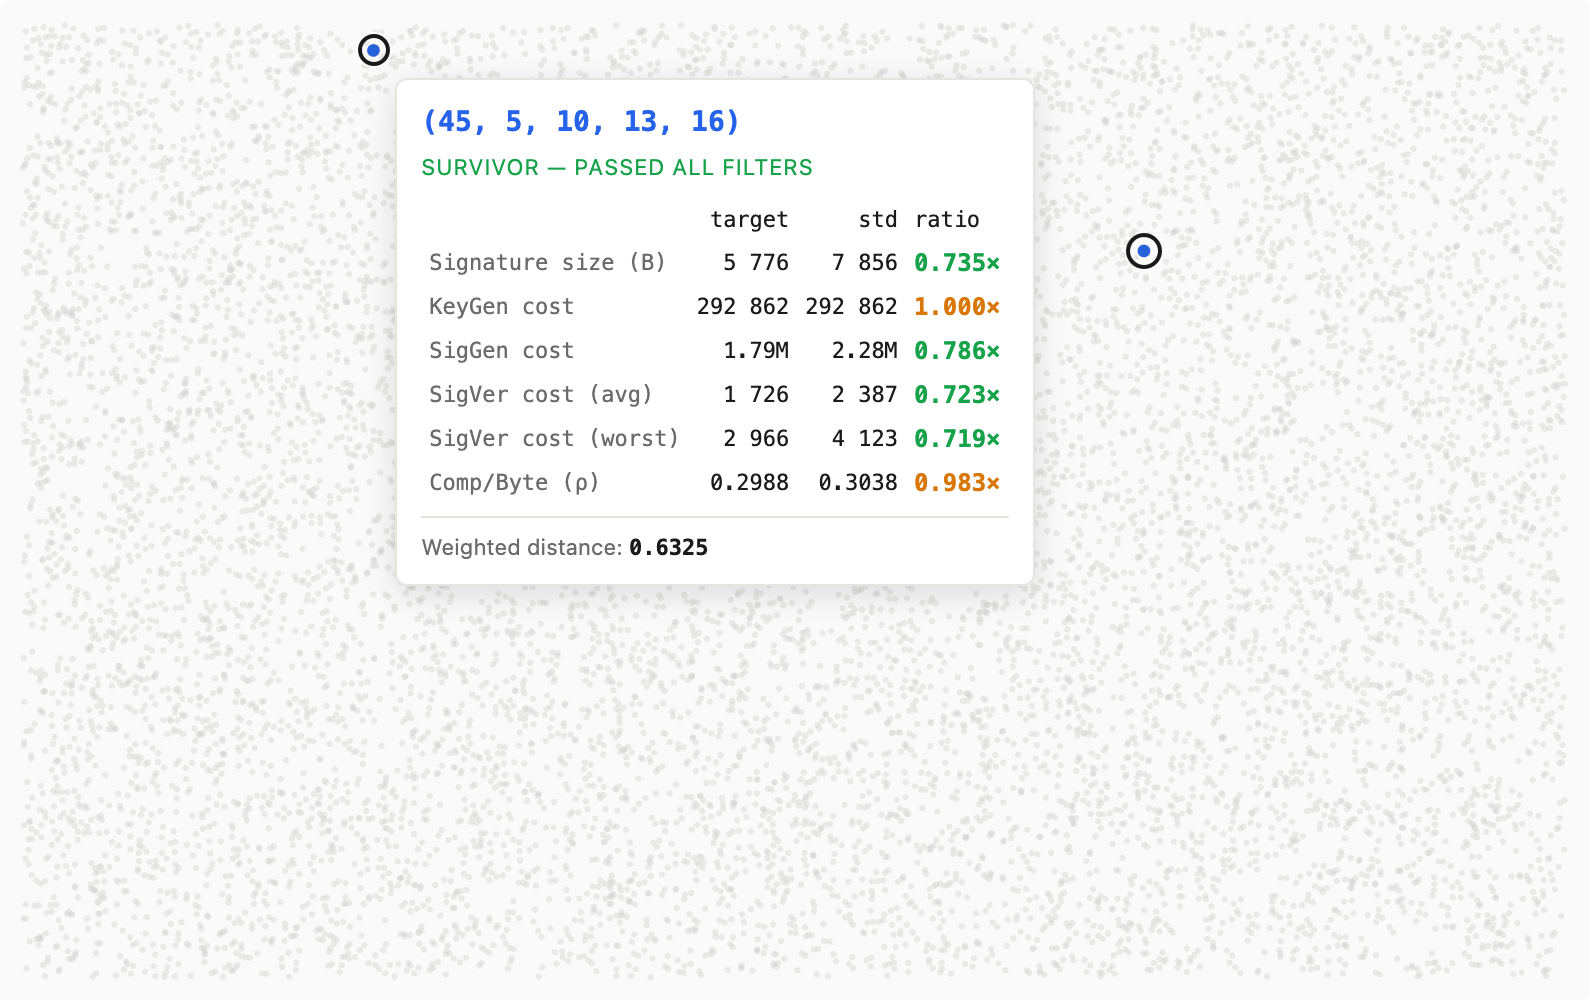
\includegraphics[width=\textwidth]{content/images/ideal_candidate_balanced.png}
        \caption{Regular weighted distance: Candidate~1 wins}
        \label{fig:ideal-balanced}
    \end{subfigure}
    \hfill
    \begin{subfigure}[b]{0.49\textwidth}
        \centering
        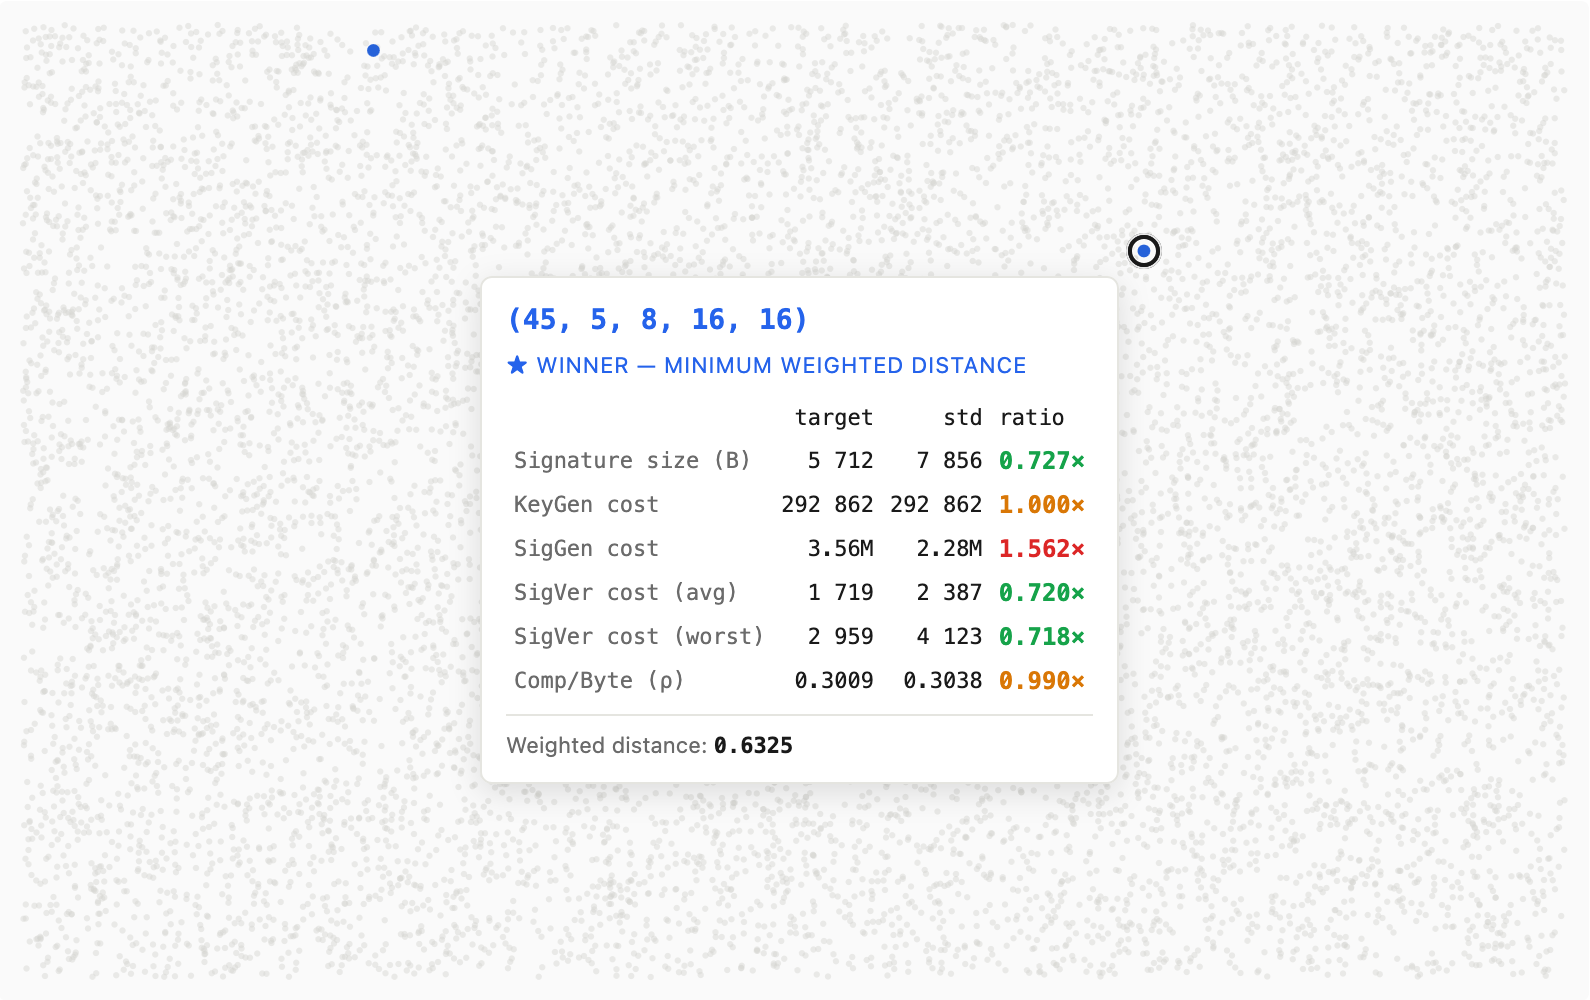
\includegraphics[width=\textwidth]{content/images/ideal_candidate_best.png}
        \caption{Metric-normalised distance degenerates to Candidate~2}
        \label{fig:ideal-best}
    \end{subfigure}
\caption{The Two Surviving Candidates under Both Distance Criteria}
\label{fig:ideal_distance_plot}
\end{figure}
